% !TeX root = ../main.tex

\chapter{引言}

\section{研究背景与意义}

随着深度学习技术的发展,深度神经网络(DNN)得到越来越广泛的应用,并在许多领域取得了超越传统算法的效果。卷积神经网络(CNN)作为一种典型的深度神经网络,在如今的计算机视觉领域获得越来越多的青睐,其在大数据规模下的图像分类、目标检测、语义分割、图像重建、人体姿态估计等任务上展现出前所未有的效果。早在2016年的经典卷积神经网络ResNet\citep{resnet}就已经在ILSVRC(ImageNet Large Scale Visual Recognition Challenge)2015比赛测试集中取得了3.57\%的Top 5错误率,超过了人类的水平。鉴于卷积神经网络在计算机视觉领域的巨大成就,因此作为深度学习模型的重要分支,卷积神经网络有着广阔的应用前景,当应用于图像识别与分割时,可用于相册图像的精准分类、零售业自动售货系统的商品识别;当应用于目标检测和人脸检测时,可用于人脸特征识别和自动驾驶的感知算法。

虽然卷积神经网络已经在计算机视觉领域表现出了巨大的应用潜力,但是应用场景的条件限制和神经网络算法资源需求量大的矛盾仍然制约着卷积神经网络算法的落地应用。目前人工智能算法的应用场景多是移动端和边缘端设备,例如手机、汽车、物联网设备等。这些应用场景有两大特点,一是计算和存储资源有限,边缘端设备为了考虑功耗、体积、成本等因素,往往采用低算力的处理器和较小容量的存储器;二是有实时性要求,卷积神经网络的感知算法需要达到甚至超过人类感知环境的速度,才能在现实中获得广泛应用,例如自动驾驶中的感知算法,出于安全性的考虑对算法实时得出结果的要求非常高。与应用场景对应,目前的深度神经网络算法有两大问题导致其难以落地应用,一是模型参数量巨大,需要大量的存储空间,例如经典图像分类网络VGG-16\citep{vgg}包含了大约个\num{1.4e8}个32位单精度浮点数参数,存储模型需要超过500MB的存储空间;二是计算量巨大,网络模型在推理时需要进行大量的二维卷积计算,具体来说是浮点数的乘加操作,上述VGG-16网络就需要进行\num{1.6e10}次浮点计算。深度神经网络部署需要大量的存储资源和计算资源,这也成为深度神经网络大规模商用的最大难题。

学术界和商业界都提出了很多方法解决深度神经网络模型资源需求过大的问题。目前主要分为模型压缩和轻量化网络设计两个方向。模型压缩是在已有网络模型的前提下,通过对模型进行调整,得到资源消耗小的新模型;轻量化网络设计则是从头开始以资源消耗小为目的设计网络。两者的最大区别是是否依赖于已有的网络模型。模型压缩由于具有良好的泛化性和硬件适应性而受到了更多的关注,主流的模型压缩方法分为低精度、量化、剪枝、蒸馏等。低精度是指将32位的单精度浮点数转换成16位或更低位数的浮点数,量化则是将32位单精度浮点数转换位8位或更低位数的定点数表示。相同数量下低位宽数据的存储空间更小,硬件计算速度也更快。剪枝是去除一些网络中的计算模块,减少网络整体计算量。蒸馏则是先仿照教师网络设计出计算量和参数量都更小的学生网络,再通过蒸馏的方法让学生网络学习到老师网络的知识,从而在推理时只使用学生网络,达到减少资源消耗的目的。其中量化是目前应用最广泛的模型压缩方法,很多硬件厂商的神经网络芯片都配置了专门用于int8量化计算的模块。普通量化将32位单精度浮点数转换为8位,量化的极限是将32位单精度浮点数转换为1位,由于1个比特位只能表示两种状态,因此这种极限的量化也称为二值化。

神经网络二值化作为模型压缩的一种方法,可以极大的减少深度神经网络算法对资源的消耗。网络在二值化时将32位的权重和激活值量化为1位,从计算角度看,原始的卷积操作是权重和激活值的32位单精度浮点数乘法和加法运算,二值化后转变为1位的乘法和加法运算,1位乘法可以用同或位运算代替,加法可以用位计数运算代替。由于位运算的硬件实现显著简单于浮点运算器,且运算速度显著高于浮点运损,因此二值化后的卷积计算可以极大的降低计算资源消耗,提升网络推理速度。有研究表明在CPU上使用位运算实现的二值卷积比浮点卷积快58倍\citep{xnornet}。从存储角度看,网络权重从32位量化为1位,直接减少了32倍的存储空间占用。因此,一旦深度神经网络二值化的技术成熟,就可以极大地降低深度学习算法落地部署的成本,使人工智能算法的大规模商用成为可能。

神经网络二值化方法的研究可以辅助理解深度神经网络的冗余性和可解释性。目前的研究表明深度神经网络中的大量连接和参数都是冗余的,神经网络的冗余性是剪枝技术的基础。神经网络逐层计算提取特征的过程是十分抽象的,整体推理过程处于黑盒状态。虽然很多研究人员尝试解释神经网络特征提取的过程,但目前仍然没办法解释。二值神经网络的实验表明,网络中的激活值和权重在1位的情况下,网络仍然可以前向推理得到结果。这不仅证实了神经网络中大量的冗余性,还可以通过观察二值特征与浮点特征的区别,对冗余性的本质分析提供线索。32位浮点特征图每个元素有大约$2^{32}$种状态,而二值化后的特征图每个元素只有2种状态。这种极度简化的特征图有利于人们进一步研究神经网络的可解释性。综上所述,神经网络二值化方法的研究可以极大地降低基于深度学习的人工智能算法商用落地的门槛,加速人工智能时代的到来,也可以为深度学习算法的理论研究提供帮助,对商业界和学术界都有着重大的意义和深远的影响。

\section{研究问题与难点}

神经网络二值化作为一种极致的量化方法,实现难度较大。以ImageNet数据集上的图像分类任务为例,如果没有加入针对二值化过程的专门设计,二值网络的Top1精度普遍要比相同结构的32位浮点网络低10\%以上。相同结构二值网络的性能较差主要有两点原因:

(1)神经网络二值化后的模型能力不足

神经网络的模型能力可以分为由激活值决定的特征表示能力和由权重决定的模型拟合能力两种。神经网络二值化需要将激活值和权重都转换为1位表示的二元状态值,因此会对神经网络的两种模型能力都产生影响。

从特征表示能力看,激活值二值化严重影响了特征图的特征表示能力。深度神经网络中每层的激活值构成了特征图,激活值从32位到1位的转换使得特征图的特征多样性直接减少了$2^{31}$倍。二值化前后的特征图可视化对比如图 \ref{fig:float_bin} 所示,可以看到二值化过程对特征图造成了大量的信息损失,并引入了大量噪声。32位浮点特征图中两个响应强度相近但不相同的特征值在二值特征图中既可能被归为一类,也可能被分为两类,无论哪种情况都会使浮点特征图的信息丢失。因此二值特征图有限的特征表示能力制约了二值神经网络的整体性能。有效的提升二值特征图的特征表示能力,是目前学术界研究的热点。

\begin{figure}[htb]
  \centering
  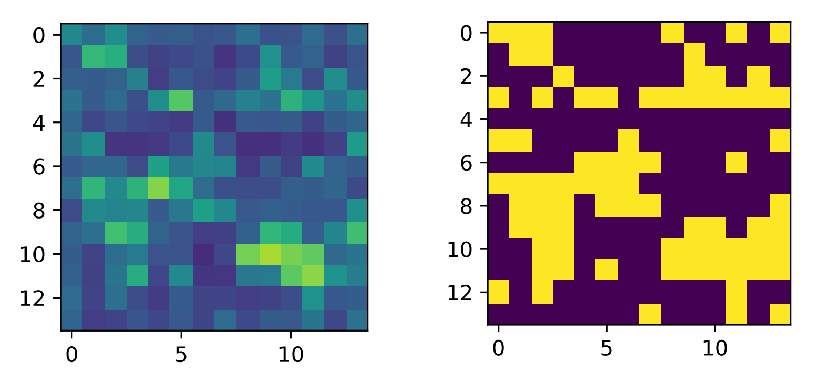
\includegraphics[width=0.6\textwidth]{float_bin.pdf}
  \caption{二值化前后的特征图可视化对比图}
  \label{fig:float_bin}
\end{figure}

从模型拟合能力看,权重二值化严重限制了网络的函数拟合能力。深度神经网络的成功来自于其优异的泛化性,通用近似定理\citep{ua}表明两层的神经网络在某些条件下即可拟合任何函数。实际的深度神经网络中数以万亿计的权重参数构成了庞大的函数空间,可以实现任意输入图像到输出类别的映射。但这种泛化性只在权重参数取值为实数时成立,当权重被量化为二元状态值时,神经网络的函数拟合能力便急剧下降。虽然依靠庞大的参数量仍然能够使二值神经网络具有解决图像分类等问题的能力,但是函数空间的缩小使得网络的优化更加困难,权重的二值化带来的泛化性降低客观上限制了二值神经网络的性能。

(2)浮点神经网络与二值神经网络对结构的需求不同

神经网络二值化将权重和激活值都从32位转换为1位,这种数值表示方式的巨大变化已经量变引起质变,极大的改变了神经网络模型的拟合函数空间。因此网络结构形式相同的浮点网络和二值网络本质上已经具有不同的网络性质。不进行结构优化的情况下将浮点网络直接转换为二值网络,将导致二值网络的性能不理想。

适合浮点网络的网络设计可能不适合二值网络。由于特征表示方式的差异,为浮点网络设计的网络结构可能无法在二值网络中使用。例如浮点网络中经常使用ReLU函数作为非线性激活函数,但是实验表明将具有ReLU函数的浮点网络直接转换为二值网络后网络训练无法收敛。这是因为二值网络激活值仅有-1和+1两种取值,ReLU函数会截断负数激活值,使特征图中+1的比例极大,网络丢失大量的特征信息。因此二值神经网络需要像轻量化网络一样专门对网络结构进行设计和改造,并对网络模块中的卷积层、激活函数层、归一化层等进行仔细的斟酌和设计,才可能实现较好的性能表现。

不适合浮点网络的网络设计可能在二值网络中发挥巨大作用。二值网络中使用的1位数的卷积提取特征,这种卷积的特征提取能力有限,在网络中添加少量的浮点操作即可显著改善网络的特征提取能力。例如XNOR-Net\cite{xnornet}等网络结构中添加的逐元素缩放因子对二值网络的性能提升有很大帮助,但是对浮点网络却几乎没有影响。设计逐元素浮点计算的网络模块可以以增加极少浮点计算量为代价显著提高二值网络的特征提取能力。二值化过程将连续的输入映射位离散的两个值,因此二值化对输入的分布十分敏感。对特征分布进行调整的网络结构在二值网络中的作用远大于在浮点网络中的作用。浮点网络和二值网络截然不同的结构需求导致很难设计通用性的神经网络二值化方法,人们需要为二值神经网络量身定制合适的模块结构。

\section{主要研究内容}

图像分类是计算机视觉领域的基本任务之一,神经网络在图像分类任务上的表现可以很好的反应网络的特征提取能力。本文主要研究如何提升二值神经网络在图像分类任务上的性能。本文的研究框架如图 \ref{fig:framework} 所示,针对1.2节的研究难点,本文从增强二值特征表示能力和设计二值友好结构两个方面进行研究,并设计了基于特征增强的二值神经网络结构。下面分别概述上述研究点。

\begin{figure}[htb]
  \vspace{6pt}
  \centering
  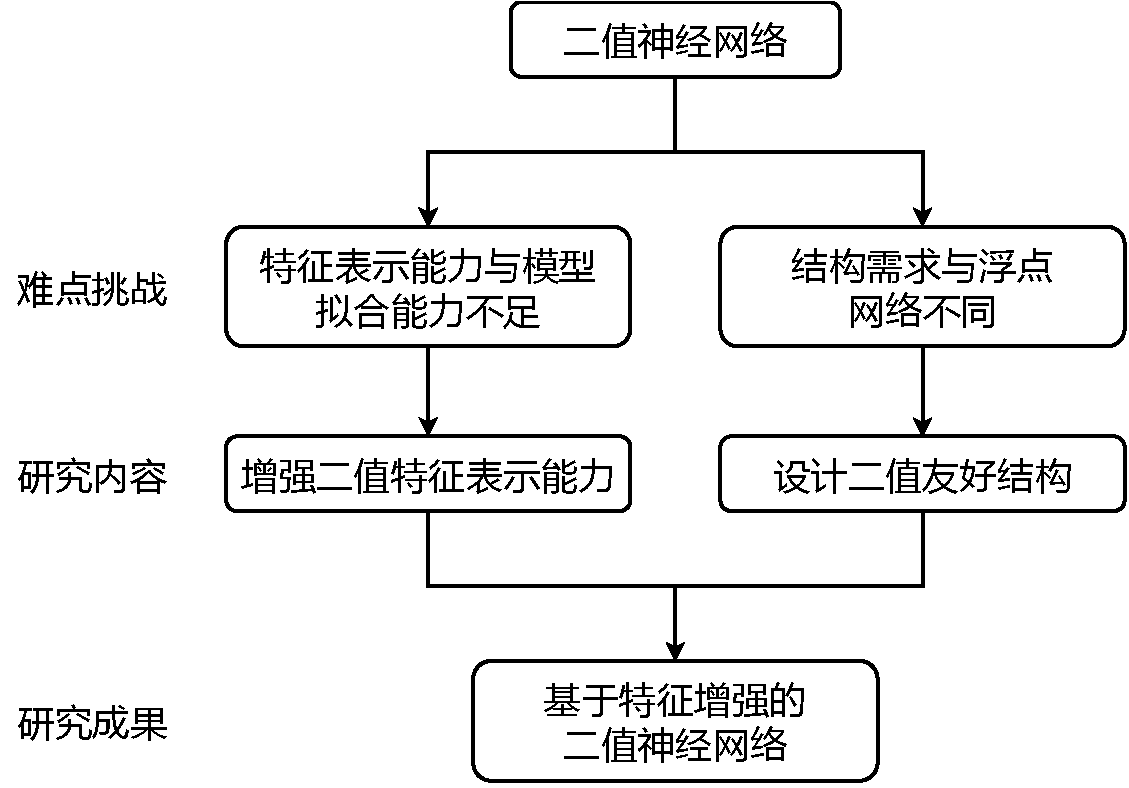
\includegraphics[width=0.8\textwidth]{framework.pdf}
  \caption{本文研究框架}
  \label{fig:framework}
\end{figure}

(1)增强二值特征表示能力

特征表示能力的不足是二值神经网络性能较差的主要原因,如何增加二值神经网络的特征表示能力是神经网络二值化领域的研究热点。多比特近似方法\citep{abcnet}可以很好的增加特征表示能力,该方法不是将激活值和权重用1位表示,而是用多位表示,只是在实际运算时应用乘法结合律将两个多位表示的数之间的乘法转换为1位乘法,也就是二值运算。使用多位表示虽然提升了特征的信息量,但是计算量也平方级增加,一定程度上抵消了二值网络计算效率高的优点。简单的增加通道数\cite{meliusnet}也可以提高网络整体特征表示能力,增加通道数会等比例的增加计算量。但是这种方法对计算量的利用率不高,这是因为神经网络中通道间相互独立,单纯的增加通道数同时也增加了冗余通道的数量,导致通道利用率没有明显提升。

针对上述方法存在的问题,本文研究如何在不增加大量计算量的情况下充分利用二值特征进而提高网络的特征表示能力。本文提出了多二值特征图方法,使用多张二值特征图来尽可能多的保留浮点特征图中的信息。多张二值特征图来源于同一张浮点特征图,可以从不同的角度保留浮点特征图中的信息,充分利用二值特征图有限的特征表示能力,不会产生冗余的计算。
在多特征图方法中,本文研究了多个二值函数的选择问题。本文使用不同阈值的符号函数作为不同二值函数从一张浮点特征图得到不同的二值特征图。为了衡量不同二值函数选取对多特征图方法的影响,本文设计了二值特征相似度作为多特征图方法中二值特征有效性的评价指标。研究\cite{unbalance}表明符号函数阈值的选取对二值网络的性能影响很大,且阈值无法随网络一同优化。本文研究了二值网络中阈值参数的性质,提出将阈值作为神经网络的结构参数看待。本文进一步研究了阈值参数的优化方法,开创性的提出阈值参数和权重参数迭代优化的方法,使自动优化的阈值可以达到手工搜索的性能水平。

(2)设计二值友好结构

二值网络受网络结构影响很大,本文从ResNet-18\cite{resnet}的结构出发,结合二值网络结构设计的成功经验,探究了二值友好的神经网络结构。为了优化梯度在二值激活值处的传递,自Bi-real Net\cite{birealnet}开始,二值网络几乎都采用了残差连接单一卷积模块的结构。本文以此为基础,进一步探究了卷积模块中的卷积层、归一化层和激活层的顺序对二值网络的影响,并对结果进行了分析。神经网络中卷积的计算量占到全部计算量的90\%以上,神经网络二值化旨在通过位操作代替卷积中的乘加操作,减少网络的计算量。由于二值卷积的特征解析能力有限,计算量占比极低的浮点逐元素操作对网络的影响力显著提升。对卷积结果的逐元素操作可以改变特征的分布,其中的浮点计算可以增强网络的特征表达能力。有方法通过专门设计的逐元素操作实现了较好的二值网络性能\cite{reactnet}。本文充分研究了逐元素操作对浮点特征的影响,提出使用分段线性缩放函数调整浮点特征的分布,增强网络的非线性性,进而提升网络整体的特征表达能力。实验表明本文提出的分段线性缩放模块可以以极少的浮点计算为代价显著提升二值神经网络的性能。

(3)基于特征增强的二值神经网络

本文将多二值特征图方法和二值友好网络结构设计方法相结合,设计了基于特征增强的二值神经网络MFNet。本文探究了多特征图方法的应用,对传统网络结构的通道数配置进行重新设置。为了最大限度地减少MFNet网络的总计算量,本文从首层卷积、升维降采样模块等方面进行设计,使MFNet充分发挥二值神经网络推理速度快的优势。

\section{论文结构}

第一章,引言。概述研究神经网络二值化方法的背景与意义,从特征表达能力和梯度不匹配两个角度分析了神经网络二值化方法的问题和难点,并总结了本文主要研究内容。

第二章,国内外研究现状。介绍了二值卷积神经网络的基本概念和实现方法,从减小量化误差、优化梯度近似、提高训练能力、设计二值友好结构等方面介绍了国内外研究现状和发展趋势。

第三章,多二值特征图方法设计。介绍本文提出的多二值特征图方法,首先概述多二值特征图方法原理,然后介绍二值特征相似度评价指标和阈值参数的设置方法,最后根据实验证明多二值特征图方法的有效性和阈值选择策略的合理性。

第四章,二值友好网络结构设计。介绍本文提出的专门适用于二值网络的模块内网络层排布顺序和模块间激活函数,通过实验验证了上述方法的有效性。

第五章,基于特征增强的二值神经网络设计。介绍组合多二值特征图方法和二值友好结构设计得到的基于特征增强的二值神经网络MFNet。详细介绍了MFNet的实现细节,并将MFNet的实验性能与其他二值网络方法进行比较。

第五章,总结与展望。总结本文的工作内容,对下一步研究工作进行展望。